% Appendix

\chapter{PLATFORM DEVELOPMENT}

During the development, there were several challenges faced:
\begin{enumerate}
    \item Distribution of the source code;
    \item Distribution of the NUIX-Studio App demos;
    \item Creating Tutorials;
    \item Providing API for external projects;
    \item Updating the dependencies;
    \item Rewriting the code to support new architectures.
\end{enumerate}

The main repository of the platform is hosted at https://github.com/VRSimulator/NUIX-Studio-Client (TODO: put the link into the references), with the previous prototypes being hosted on other repositories.

The distribution of the source code and the NUIX-Studio App demos required keeping the size of the repository at minimum, while providing an easy installation procedure. To follow these requirements, NUIX-Studio was shared as a separate package, possible to integrate into any Unity project.

The first prototypes of the NUIX-Studio platform did not support Virtual reality (Figure~\ref{fig:Prototype2-figure}), and were based on a different architecture (Figure~\ref{fig:Prototype3Structure-figure}).


\begin{figure}
  \centering
  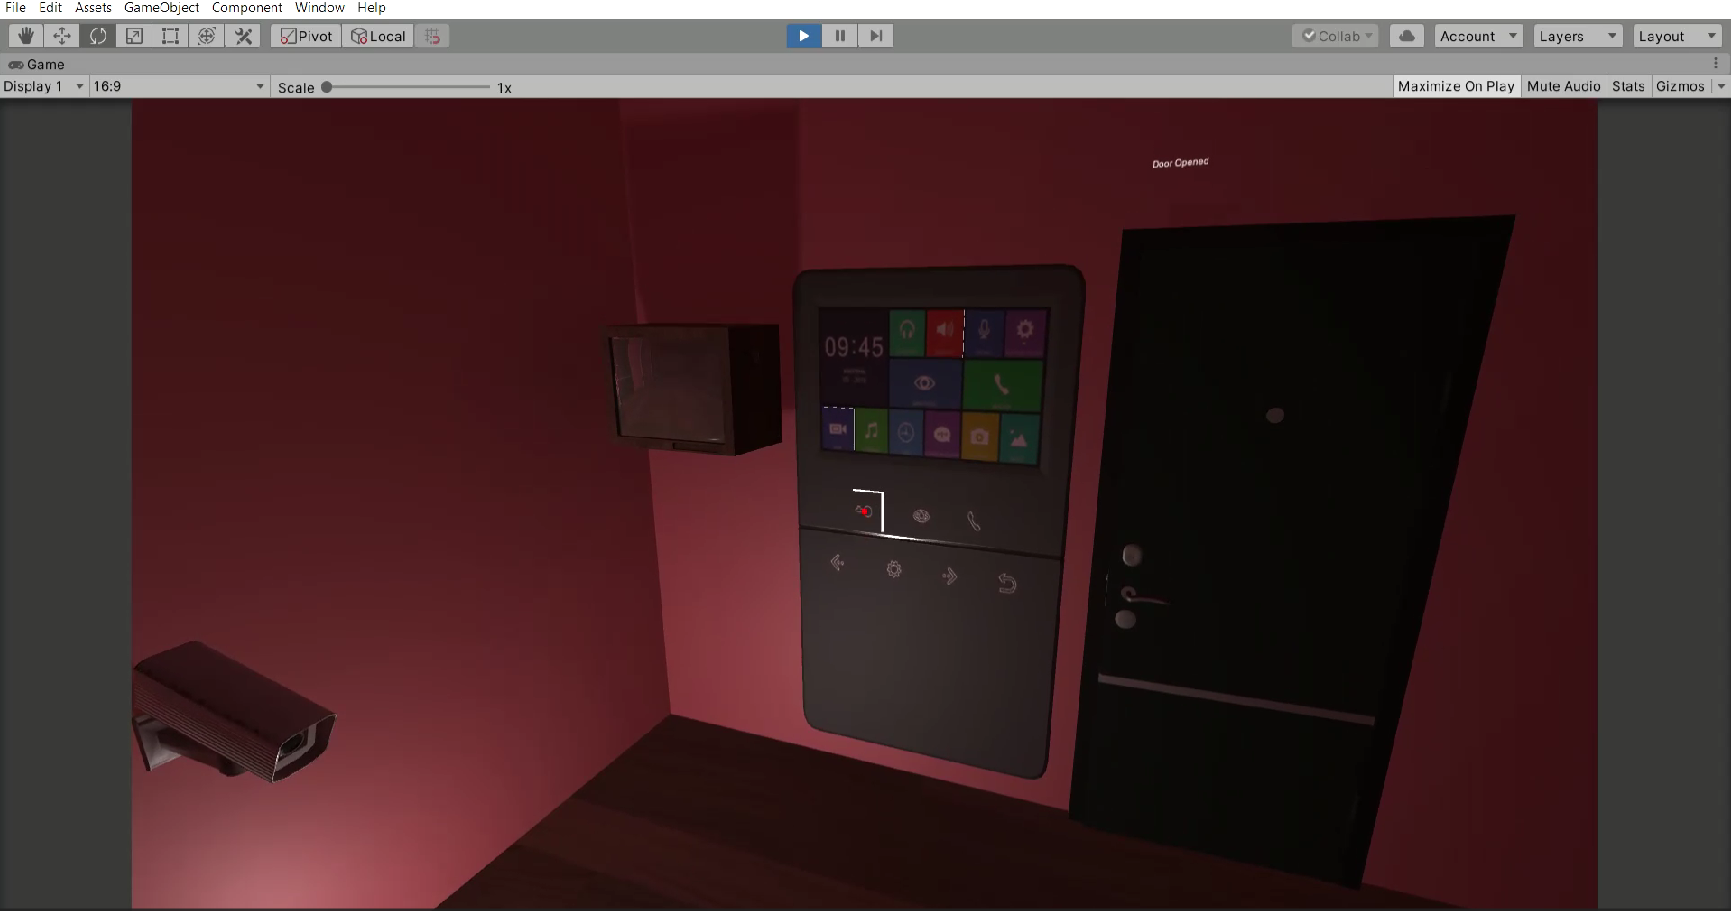
\includegraphics[width=0.6\linewidth]{figures/Prototype2.png}
  \caption{The second prototype of the VR-IoT Research platform}
  \label{fig:Prototype2-figure}
\end{figure}

\begin{figure}
  \centering
  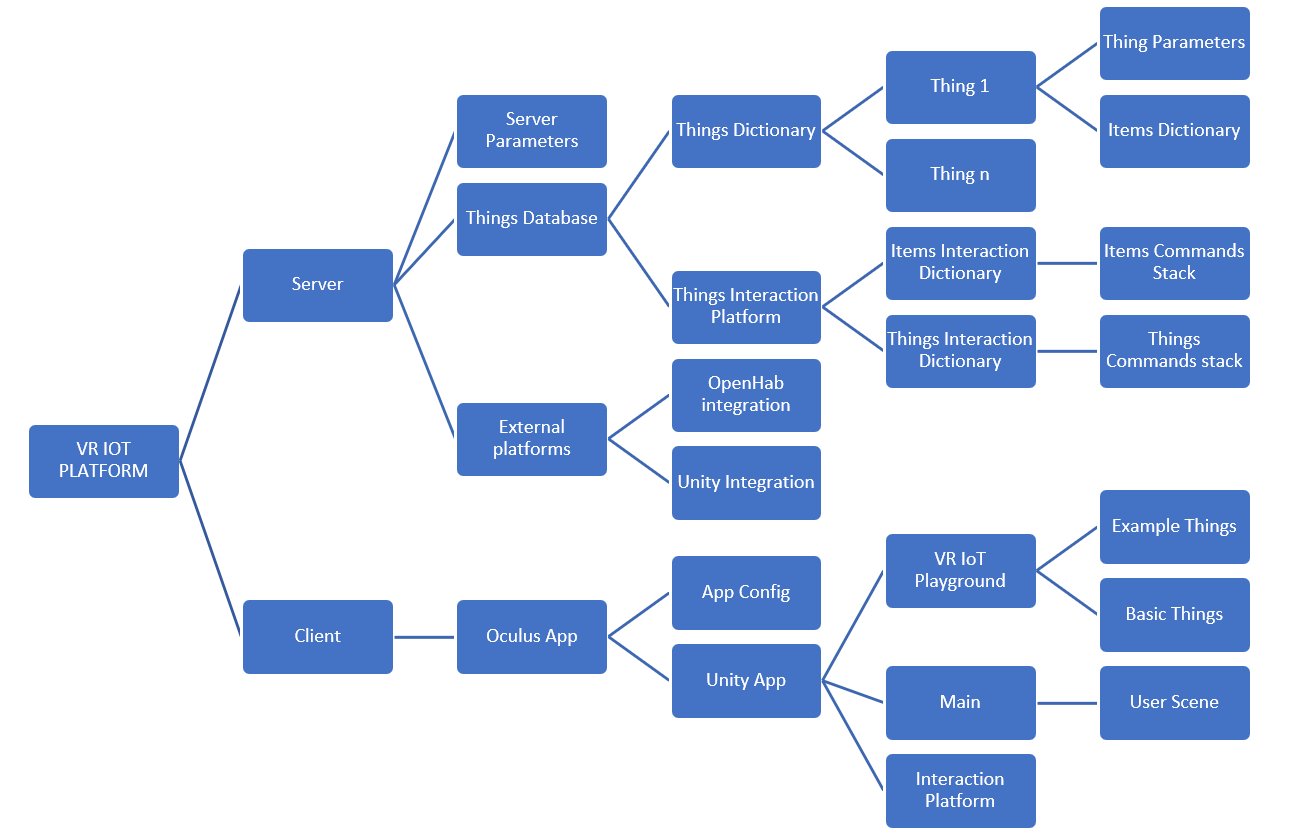
\includegraphics[width=0.9\linewidth]{figures/Prototype3Structure.png}
  \caption{The third prototype's structure}
  \label{fig:Prototype3Structure-figure}
\end{figure}

The difference between the final structure used in NUIX-Studio and the structure in Figure~\ref{fig:Prototype3Structure-figure} is in the way the data is stored on the server. In the previous prototypes the server was responsible not only for storing and synchronizing item parameters, but also for keeping all the Unity-specific functionality in a separate framework. This framework was responsible for building Item representations for virtual reality and sharing them to other NUIX-Studio App instances as Unity Gameobjects. The main limitation of this approach is that Unity Gameobjects have much bigger size compared to the Data transfer objects used in the final prototype.

\begin{figure}
  \centering
  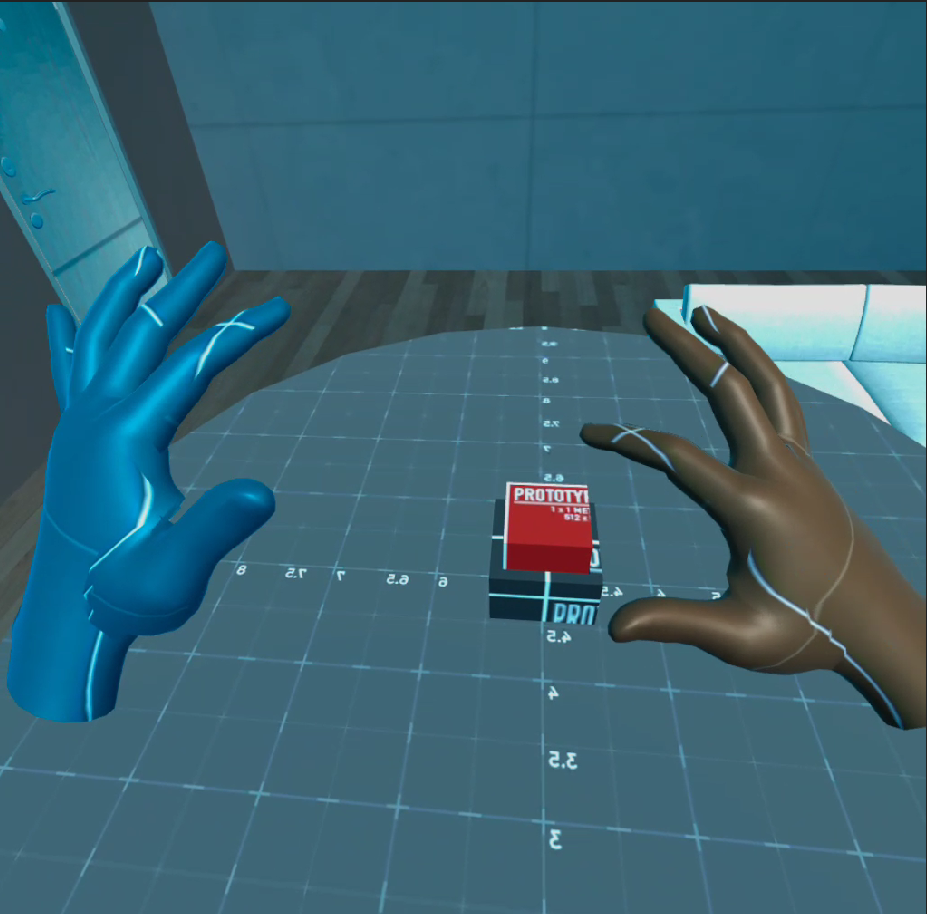
\includegraphics[width=0.6\linewidth]{figures/Prototype3.png}
  \caption{The third prototype of the VR-IoT Research platform. Button Widget.}
  \label{fig:Prototype3-figure}
\end{figure}

The third prototype provided only a button Widget (Figure~\ref{fig:Prototype3-figure}), but after integrating Mixed Reality Toolkit in the fourth prototype (Figure~\ref{fig:Prototype4-figure}), other Widgets were added to the platform.

\begin{figure}
  \centering
  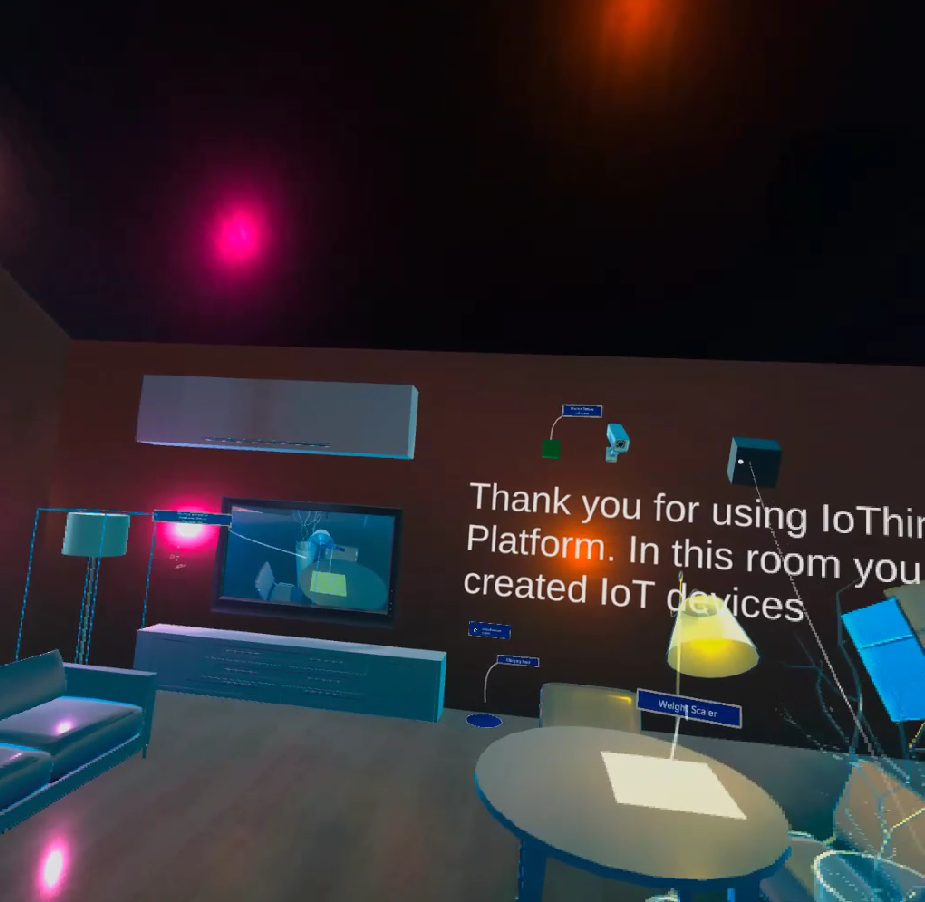
\includegraphics[width=0.6\linewidth]{figures/Prototype4.png}
  \caption{The fourth prototype of the VR-IoT Research platform. A virtual copy of the real-world smart home environment was used with virtual items added, such as location item, contact item, player item switch item, and dimmer item. Also several Widgets were supported: sight sensor, motor, light widget, pressure sensor, video streaming screens and gesture recognition.}
  \label{fig:Prototype4-figure}
\end{figure}

In the final prototype (Figure~\ref{fig:FinalPrototype-figure}), code for most of the items was rewritten to support the new architecture. 

\begin{figure}
  \centering
  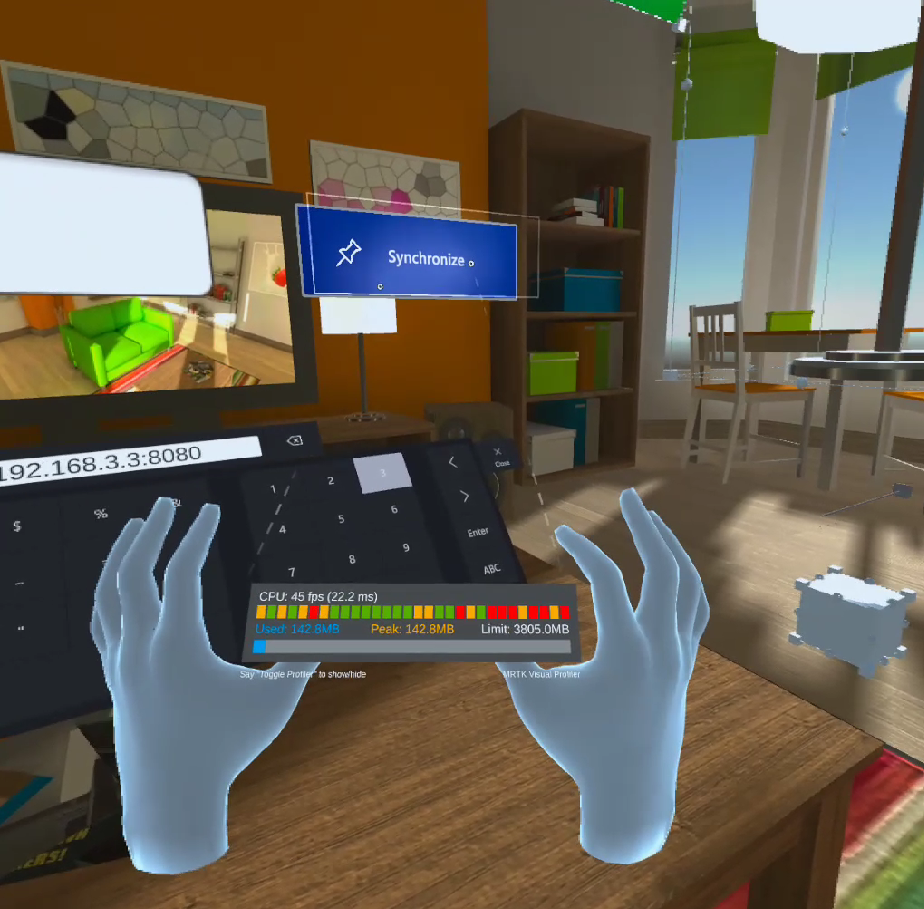
\includegraphics[width=0.6\linewidth]{figures/FinalPrototype.png}
  \caption{Screenshot of the final prototype of NUIX-Studio.}
  \label{fig:FinalPrototype-figure}
\end{figure}